%%%% Paramétrage du TD %%%%
\def\xxactivite{ \ifprof \normalsize{TD 4 -- Corrigé } \else  \ifcolle Colle \else TD 4\fi \fi} % \normalsize \vspace{-.4cm}
\def\xxauteur{\textsl{Xavier Pessoles}}

\def\xxnumchapitre{Chapitre 2 \vspace{.2cm}}
\def\xxchapitre{\hspace{.12cm} Hyperstatisme}



\def\xxcompetences{%
\vspace{-.5cm}
\footnotesize{
\textsl{%
\textbf{Savoirs et compétences :}\\
\vspace{-.2cm}
\begin{itemize}[label=\ding{112},font=\color{ocre}] 
%\item \textit{Mod2.C34} : chaînes de solides;
\item \textit{Mod2.C34} : degré de mobilité du modèle;
\item \textit{Mod2.C34} : degré d’hyperstatisme du modèle;
\item \textit{Mod2.C34.SF1} : déterminer les conditions géométriques associées à l’hyperstatisme;
\item \textit{Mod2.C34} : résoudre le système associé à la fermeture cinématique et en déduire le degré de mobilité et d’hyperstatisme.
\end{itemize}}}}

\def\xxtitreexo{Tuyère à ouverture variable}
\def\xxsourceexo{\hspace{.2cm} \footnotesize{Banque PT -- SIA 2011}}

\def\xxfigures{
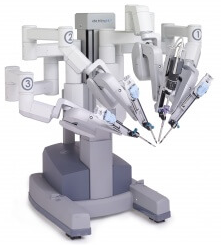
\includegraphics[width=.75\textwidth]{fig_00}
}%figues de la page de garde




\iflivret
\pagestyle{empty}


%%%%%%%% PAGE DE GARDE COURS
\ifcours
\begin{tikzpicture}[remember picture,overlay]
\node at (current page.north west)
{\begin{tikzpicture}[remember picture,overlay]
\node[anchor=north west,inner sep=0pt] at (0,0) {\includegraphics[width=\paperwidth]{\thechapterimage}};
\draw[anchor=west] (-2cm,-8cm) node [line width=2pt,rounded corners=15pt,draw=ocre,fill=white,fill opacity=0.6,inner sep=40pt]{\strut\makebox[22cm]{}};
\draw[anchor=west] (1cm,-8cm) node {\huge\sffamily\bfseries\color{black} %
\begin{minipage}{1cm}
\rotatebox{90}{\LARGE\sffamily\textsc{\color{ocre}\textbf{\xxnumpartie}}}
\end{minipage} \hfill
\begin{minipage}[c]{14cm}
\begin{titrepartie}
\begin{flushright}
\renewcommand{\baselinestretch}{1.1} 
\Large\sffamily\textsc{\textbf{\xxpartie}}
\renewcommand{\baselinestretch}{1} 
\end{flushright}
\end{titrepartie}
\end{minipage} \hfill
\begin{minipage}[c]{3.5cm}
{\large\sffamily\textsc{\textbf{\color{ocre} \discipline}}}
\end{minipage} 
 };
\end{tikzpicture}};
\end{tikzpicture}


\begin{tikzpicture}[overlay]
\node[shape=rectangle, 
      rounded corners = .25 cm,
	  draw= ocre,
	  line width=2pt, 
	  fill = ocre!10,
	  minimum width  = 2.5cm,
	  minimum height = 3cm,] at (18cm,0) {};
\node at (17.7cm,0) {\rotatebox{90}{\textbf{\Large\color{ocre}{\classe}}}};
%{};
\end{tikzpicture}

\vspace{3.5cm}

\begin{tikzpicture}[remember picture,overlay]
\draw[anchor=west] (-2cm,-6cm) node {\huge\sffamily\bfseries\color{black} %
\begin{minipage}{2cm}
\begin{center}
\LARGE\sffamily\textsc{\color{ocre}\textbf{\xxactivite}}
\end{center}
\end{minipage} \hfill
\begin{minipage}[c]{15cm}
\begin{titrechapitre}
\renewcommand{\baselinestretch}{1.1} 
\Large\sffamily\textsc{\textbf{\xxnumchapitre}}

\Large\sffamily\textsc{\textbf{\xxchapitre}}
\vspace{.5cm}

\renewcommand{\baselinestretch}{1} 
\normalsize\normalfont
\xxcompetences
\end{titrechapitre}
\end{minipage}  };
\end{tikzpicture}
\vfill

\begin{flushright}
\begin{minipage}[c]{.3\linewidth}
\begin{center}
\xxfigures
\end{center}
\end{minipage}\hfill
\begin{minipage}[c]{.6\linewidth}
\startcontents
\printcontents{}{1}{}
\end{minipage}
\end{flushright}

\begin{tikzpicture}[remember picture,overlay]
\draw[anchor=west] (4.5cm,-.7cm) node {
\begin{minipage}[c]{.2\linewidth}
\begin{flushright}

\includegraphics[width=2cm]{png/logoCC}
\end{flushright}
\end{minipage}
\begin{minipage}[c]{.2\linewidth}
\textsl{\xxauteur} \\
\textsl{\classe}
\end{minipage}
 };
\end{tikzpicture}
\newpage
\pagestyle{fancy}

\newpage
\pagestyle{fancy}

\else
\fi


%%%%%%%% PAGE DE GARDE TD
\iftd
%\begin{tikzpicture}[remember picture,overlay]
%\node at (current page.north west)
%{\begin{tikzpicture}[remember picture,overlay]
%\draw[anchor=west] (-2cm,-3.25cm) node [line width=2pt,rounded corners=15pt,draw=ocre,fill=white,fill opacity=0.6,inner sep=40pt]{\strut\makebox[22cm]{}};
%\draw[anchor=west] (1cm,-3.25cm) node {\huge\sffamily\bfseries\color{black} %
%\begin{minipage}{1cm}
%\rotatebox{90}{\LARGE\sffamily\textsc{\color{ocre}\textbf{\xxnumpartie}}}
%\end{minipage} \hfill
%\begin{minipage}[c]{13.5cm}
%\begin{titrepartie}
%\begin{flushright}
%\renewcommand{\baselinestretch}{1.1} 
%\Large\sffamily\textsc{\textbf{\xxpartie}}
%\renewcommand{\baselinestretch}{1} 
%\end{flushright}
%\end{titrepartie}
%\end{minipage} \hfill
%\begin{minipage}[c]{3.5cm}
%{\large\sffamily\textsc{\textbf{\color{ocre} \discipline}}}
%\end{minipage} 
% };
%\end{tikzpicture}};
%\end{tikzpicture}

%%%%%%%%%% PAGE DE GARDE TD %%%%%%%%%%%%%%%
%\begin{tikzpicture}[overlay]
%\node[shape=rectangle, 
%      rounded corners = .25 cm,
%	  draw= ocre,
%	  line width=2pt, 
%	  fill = ocre!10,
%	  minimum width  = 2.5cm,
%	  minimum height = 2.5cm,] at (18.5cm,0) {};
%\node at (17.7cm,0) {\rotatebox{90}{\textbf{\Large\color{ocre}{\classe}}}};
%%{};
%\end{tikzpicture}

% PARTIE ET CHAPITRE
%\begin{tikzpicture}[remember picture,overlay]
%\draw[anchor=west] (-1cm,-2.1cm) node {\large\sffamily\bfseries\color{black} %
%\begin{minipage}[c]{15cm}
%\begin{flushleft}
%\xxnumchapitre \\
%\xxchapitre
%\end{flushleft}
%\end{minipage}  };
%\end{tikzpicture}

% Bandeau titre exo
\begin{tikzpicture}[remember picture,overlay]
\draw[anchor=west] (-2cm,-4cm) node {\huge\sffamily\bfseries\color{black} %
\begin{minipage}{5cm}
\begin{center}
\LARGE\sffamily\color{ocre}\textbf{\textsc{\xxactivite}}

\begin{center}
\xxfigures
\end{center}

\end{center}
\end{minipage} \hfill
\begin{minipage}[c]{12cm}
\begin{titrechapitre}
\renewcommand{\baselinestretch}{1.1} 
\large\sffamily\textbf{\textsc{\xxtitreexo}}

\small\sffamily{\textbf{\textit{\color{black!70}\xxsourceexo}}}
\vspace{.5cm}

\renewcommand{\baselinestretch}{1} 
\normalsize\normalfont
\xxcompetences
\end{titrechapitre}
\end{minipage}  };
\end{tikzpicture}

\else
\fi


%%%%%%%% PAGE DE GARDE FICHE
\iffiche
\begin{tikzpicture}[remember picture,overlay]
\node at (current page.north west)
{\begin{tikzpicture}[remember picture,overlay]
\draw[anchor=west] (-2cm,-3.25cm) node [line width=2pt,rounded corners=15pt,draw=ocre,fill=white,fill opacity=0.6,inner sep=40pt]{\strut\makebox[22cm]{}};
\draw[anchor=west] (1cm,-3.25cm) node {\huge\sffamily\bfseries\color{black} %
\begin{minipage}{1cm}
\rotatebox{90}{\LARGE\sffamily\textsc{\color{ocre}\textbf{\xxnumpartie}}}
\end{minipage} \hfill
\begin{minipage}[c]{14cm}
\begin{titrepartie}
\begin{flushright}
\renewcommand{\baselinestretch}{1.1} 
\large\sffamily\textsc{\textbf{\xxpartie} \\} 

\vspace{.2cm}

\normalsize\sffamily\textsc{\textbf{\xxnumchapitre -- \xxchapitre}}
\renewcommand{\baselinestretch}{1} 
\end{flushright}
\end{titrepartie}
\end{minipage} \hfill
\begin{minipage}[c]{3.5cm}
{\large\sffamily\textsc{\textbf{\color{ocre} \discipline}}}
\end{minipage} 
 };
\end{tikzpicture}};
\end{tikzpicture}


\begin{tikzpicture}[overlay]
\node[shape=rectangle, 
      rounded corners = .25 cm,
	  draw= ocre,
	  line width=2pt, 
	  fill = ocre!10,
	  minimum width  = 2.5cm,
	  minimum height = 2.5cm,] at (18.5cm,0.5cm) {};
%	  minimum height = 2.5cm,] at (18.5cm,0cm) {};
\node at (17.7cm,0.5) {\rotatebox{90}{\textsf{\textbf{\large\color{ocre}{\classe}}}}};
%{};
\end{tikzpicture}



\else
\fi



\else
\pagestyle{empty}


%%%%%%%% PAGE DE GARDE COURS
\ifcours
\begin{tikzpicture}[remember picture,overlay]
\node at (current page.north west)
{\begin{tikzpicture}[remember picture,overlay]
\node[anchor=north west,inner sep=0pt] at (0,0) {\includegraphics[width=\paperwidth]{\thechapterimage}};
\draw[anchor=west] (-2cm,-8cm) node [line width=2pt,rounded corners=15pt,draw=ocre,fill=white,fill opacity=0.6,inner sep=40pt]{\strut\makebox[22cm]{}};
\draw[anchor=west] (1cm,-8cm) node {\huge\sffamily\bfseries\color{black} %
\begin{minipage}{1cm}
\rotatebox{90}{\LARGE\sffamily\textsc{\color{ocre}\textbf{\xxnumpartie}}}
\end{minipage} \hfill
\begin{minipage}[c]{14cm}
\begin{titrepartie}
\begin{flushright}
\renewcommand{\baselinestretch}{1.1} 
\Large\sffamily\textsc{\textbf{\xxpartie}}
\renewcommand{\baselinestretch}{1} 
\end{flushright}
\end{titrepartie}
\end{minipage} \hfill
\begin{minipage}[c]{3.5cm}
{\large\sffamily\textsc{\textbf{\color{ocre} \discipline}}}
\end{minipage} 
 };
\end{tikzpicture}};
\end{tikzpicture}


\begin{tikzpicture}[overlay]
\node[shape=rectangle, 
      rounded corners = .25 cm,
	  draw= ocre,
	  line width=2pt, 
	  fill = ocre!10,
	  minimum width  = 2.5cm,
	  minimum height = 3cm,] at (18cm,0) {};
\node at (17.7cm,0) {\rotatebox{90}{\textbf{\Large\color{ocre}{\classe}}}};
%{};
\end{tikzpicture}

\vspace{3.5cm}

\begin{tikzpicture}[remember picture,overlay]
\draw[anchor=west] (-2cm,-6cm) node {\huge\sffamily\bfseries\color{black} %
\begin{minipage}{2cm}
\begin{center}
\LARGE\sffamily\textsc{\color{ocre}\textbf{\xxactivite}}
\end{center}
\end{minipage} \hfill
\begin{minipage}[c]{15cm}
\begin{titrechapitre}
\renewcommand{\baselinestretch}{1.1} 
\Large\sffamily\textsc{\textbf{\xxnumchapitre}}

\Large\sffamily\textsc{\textbf{\xxchapitre}}
\vspace{.5cm}

\renewcommand{\baselinestretch}{1} 
\normalsize\normalfont
\xxcompetences
\end{titrechapitre}
\end{minipage}  };
\end{tikzpicture}
\vfill

\begin{flushright}
\begin{minipage}[c]{.3\linewidth}
\begin{center}
\xxfigures
\end{center}
\end{minipage}\hfill
\begin{minipage}[c]{.6\linewidth}
\startcontents
\printcontents{}{1}{}
\end{minipage}
\end{flushright}

\begin{tikzpicture}[remember picture,overlay]
\draw[anchor=west] (4.5cm,-.7cm) node {
\begin{minipage}[c]{.2\linewidth}
\begin{flushright}

\includegraphics[width=2cm]{png/logoCC}
\end{flushright}
\end{minipage}
\begin{minipage}[c]{.2\linewidth}
\textsl{\xxauteur} \\
\textsl{\classe}
\end{minipage}
 };
\end{tikzpicture}
\newpage
\pagestyle{fancy}

\newpage
\pagestyle{fancy}

\else
\fi


%%%%%%%% PAGE DE GARDE TD
\iftd
%\begin{tikzpicture}[remember picture,overlay]
%\node at (current page.north west)
%{\begin{tikzpicture}[remember picture,overlay]
%\draw[anchor=west] (-2cm,-3.25cm) node [line width=2pt,rounded corners=15pt,draw=ocre,fill=white,fill opacity=0.6,inner sep=40pt]{\strut\makebox[22cm]{}};
%\draw[anchor=west] (1cm,-3.25cm) node {\huge\sffamily\bfseries\color{black} %
%\begin{minipage}{1cm}
%\rotatebox{90}{\LARGE\sffamily\textsc{\color{ocre}\textbf{\xxnumpartie}}}
%\end{minipage} \hfill
%\begin{minipage}[c]{13.5cm}
%\begin{titrepartie}
%\begin{flushright}
%\renewcommand{\baselinestretch}{1.1} 
%\Large\sffamily\textsc{\textbf{\xxpartie}}
%\renewcommand{\baselinestretch}{1} 
%\end{flushright}
%\end{titrepartie}
%\end{minipage} \hfill
%\begin{minipage}[c]{3.5cm}
%{\large\sffamily\textsc{\textbf{\color{ocre} \discipline}}}
%\end{minipage} 
% };
%\end{tikzpicture}};
%\end{tikzpicture}

%%%%%%%%%% PAGE DE GARDE TD %%%%%%%%%%%%%%%
%\begin{tikzpicture}[overlay]
%\node[shape=rectangle, 
%      rounded corners = .25 cm,
%	  draw= ocre,
%	  line width=2pt, 
%	  fill = ocre!10,
%	  minimum width  = 2.5cm,
%	  minimum height = 2.5cm,] at (18.5cm,0) {};
%\node at (17.7cm,0) {\rotatebox{90}{\textbf{\Large\color{ocre}{\classe}}}};
%%{};
%\end{tikzpicture}

% PARTIE ET CHAPITRE
%\begin{tikzpicture}[remember picture,overlay]
%\draw[anchor=west] (-1cm,-2.1cm) node {\large\sffamily\bfseries\color{black} %
%\begin{minipage}[c]{15cm}
%\begin{flushleft}
%\xxnumchapitre \\
%\xxchapitre
%\end{flushleft}
%\end{minipage}  };
%\end{tikzpicture}

% Bandeau titre exo
\begin{tikzpicture}[remember picture,overlay]
\draw[anchor=west] (-2cm,-4cm) node {\huge\sffamily\bfseries\color{black} %
\begin{minipage}{5cm}
\begin{center}
\LARGE\sffamily\color{ocre}\textbf{\textsc{\xxactivite}}

\begin{center}
\xxfigures
\end{center}

\end{center}
\end{minipage} \hfill
\begin{minipage}[c]{12cm}
\begin{titrechapitre}
\renewcommand{\baselinestretch}{1.1} 
\large\sffamily\textbf{\textsc{\xxtitreexo}}

\small\sffamily{\textbf{\textit{\color{black!70}\xxsourceexo}}}
\vspace{.5cm}

\renewcommand{\baselinestretch}{1} 
\normalsize\normalfont
\xxcompetences
\end{titrechapitre}
\end{minipage}  };
\end{tikzpicture}

\else
\fi


%%%%%%%% PAGE DE GARDE FICHE
\iffiche
\begin{tikzpicture}[remember picture,overlay]
\node at (current page.north west)
{\begin{tikzpicture}[remember picture,overlay]
\draw[anchor=west] (-2cm,-3.25cm) node [line width=2pt,rounded corners=15pt,draw=ocre,fill=white,fill opacity=0.6,inner sep=40pt]{\strut\makebox[22cm]{}};
\draw[anchor=west] (1cm,-3.25cm) node {\huge\sffamily\bfseries\color{black} %
\begin{minipage}{1cm}
\rotatebox{90}{\LARGE\sffamily\textsc{\color{ocre}\textbf{\xxnumpartie}}}
\end{minipage} \hfill
\begin{minipage}[c]{14cm}
\begin{titrepartie}
\begin{flushright}
\renewcommand{\baselinestretch}{1.1} 
\large\sffamily\textsc{\textbf{\xxpartie} \\} 

\vspace{.2cm}

\normalsize\sffamily\textsc{\textbf{\xxnumchapitre -- \xxchapitre}}
\renewcommand{\baselinestretch}{1} 
\end{flushright}
\end{titrepartie}
\end{minipage} \hfill
\begin{minipage}[c]{3.5cm}
{\large\sffamily\textsc{\textbf{\color{ocre} \discipline}}}
\end{minipage} 
 };
\end{tikzpicture}};
\end{tikzpicture}


\begin{tikzpicture}[overlay]
\node[shape=rectangle, 
      rounded corners = .25 cm,
	  draw= ocre,
	  line width=2pt, 
	  fill = ocre!10,
	  minimum width  = 2.5cm,
	  minimum height = 2.5cm,] at (18.5cm,0.5cm) {};
%	  minimum height = 2.5cm,] at (18.5cm,0cm) {};
\node at (17.7cm,0.5) {\rotatebox{90}{\textsf{\textbf{\large\color{ocre}{\classe}}}}};
%{};
\end{tikzpicture}



\else
\fi



\fi
\setlength{\columnseprule}{.1pt}

\pagestyle{fancy}
\thispagestyle{plain}

\ifprof
\vspace{5cm}
\else
\vspace{5cm}
\fi

\def\columnseprulecolor{\color{ocre}}
\setlength{\columnseprule}{0.4pt} 

%%%%%%%%%%%%%%%%%%%%%%%

\setcounter{exo}{0}


\ifprof
\else
\begin{multicols}{2}
\fi
\section*{Mise en situation}
Dans le but de calibrer un banc d'essai de turboréacteur, les ingénieurs de la DGA (Direction Générale de l'Armement) a conçu une tuyère à ouverture variable afin de se substituer au turboréacteur. 
\begin{center}
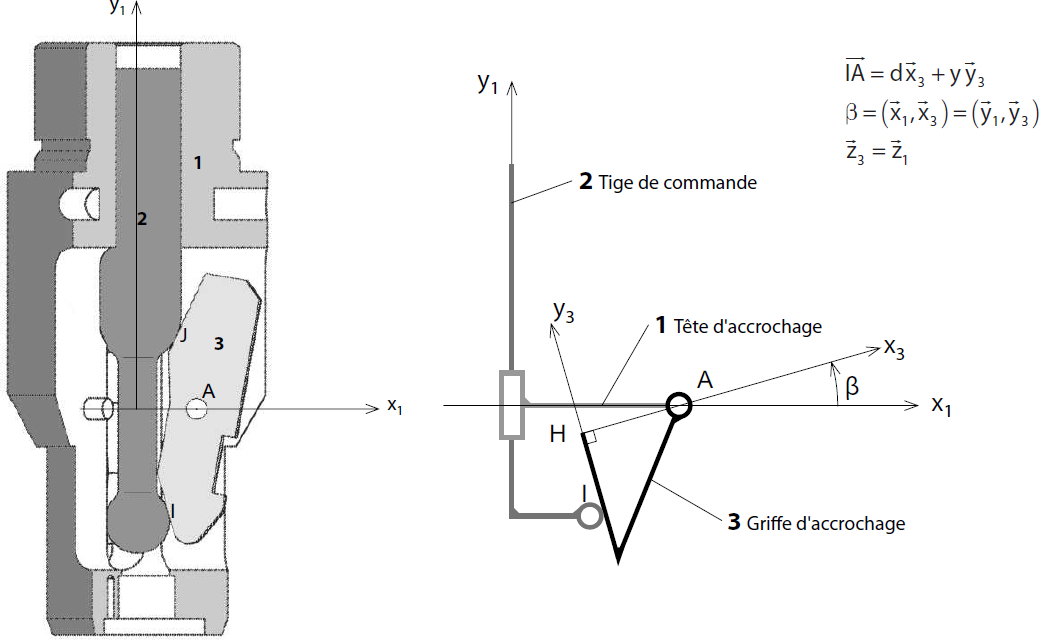
\includegraphics[width=\linewidth]{fig_01}
%\textit{}
\end{center}


\begin{obj}
L'objectif est de valider le choix de conception de la structure mécanique permettant
de transmettre l'énergie mécanique aux volets.
\end{obj}

Le mouvement de chacun des volets doit être identique. Pour cela, les exigences suivantes doivent être vérifiées :
\begin{itemize}
\item le mouvement de rotation des volets autour d'un axe orthogonal à l'axe de la veine fluide doit respecter les exigences suivantes : 
\begin{itemize}
\item position de l'axe de rotation : orthogonal;
\item débattement angulaire : 40\degres $\pm$ 0,5\degres;
\item précision angulaire : 0,2\degres;
\end{itemize}
\item commande simultanée des 16 volets :
\begin{itemize}
\item interface unique en liaison glissière par rapport à la tuyère;
\item nombre d'actionneurs : minimum;
\item rigidité globale : $\Delta x < \SI{0,2}{mm}$;
\item temps de montée en vitesse : inférieur à \SI{0,1}{s}.
\end{itemize}
\item adaptation aux efforts aérodynamiques :
\begin{itemize}
\item résistance : 50\% de la limite élastique;
\item déformation : compatible avec la précision.
\end{itemize}
\end{itemize}


La figure suivante présente les éléments de la solution adoptée par le bureau d'étude.
\begin{center}
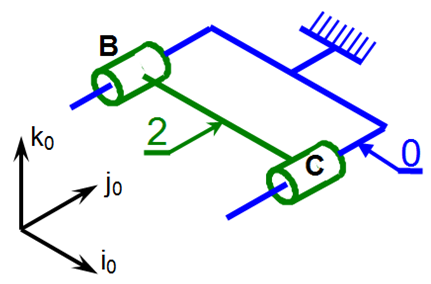
\includegraphics[width=\linewidth]{fig_02}
%\textit{}
\end{center}

Pour synchroniser la commande des volets, on a adopté une solution consistant à les relier à une pièce unique
en forme de tore entourant la tuyère et dont le déplacement assure la commande de tous les volets
simultanément. Le tore repose sur deux barres de guidage fixées dans la partie supérieure du carter et
parallèles à l'axe de la tuyère. Il est actionné par quatre vérins hydrauliques.
On cherche, dans cette partie, à valider le critère d'appréciation sur la rigidité globale de la structure de
commande des volets à interface unique.

Les notations adoptées sont les suivantes.

La base orthonormée directe liée au solide $i$: $\mathcal{B}_i = \left(\vect{x_i},\vect{y_i},\vect{z_i}\right)$. Le torseur cinématique du mouvement possible par une liaison $L_k$, d’un solide $j$ par rapport à un solide $i$
(ou par rapport au référentiel $\mathcal{R}_i$ lié à celui-ci) réduit en $A$, sera noté $\left\{ \mathcal{V}_k\right\}=\torseurl{p_k \vect{x}+q_k\vect{y}+r_k\vect{z}}{u_k \vect{x}+v_k\vect{y}+w_k\vect{z}}{A}$ où $\left(\vect{x},\vect{y},\vect{z}\right)$ est une base orthonormée associée à la liaison $L_k$. 

Le torseur des actions mécaniques transmissibles par la liaison $L_k$ du solide $i$ sur le solide $j$, réduit en $A$ sera noté $\left\{ \mathcal{F}_k\right\}=\torseurl{X_k \vect{x}+Y_k\vect{y}+Z_k\vect{z}}{L_k \vect{x}+M_k\vect{y}+N_k\vect{z}}{A}$ où $\left(\vect{x},\vect{y},\vect{z}\right)$ est une base orthonormée associée à la liaison $L_k$. 

\subsection*{Étude d'une commande avec un seul actionneur}

\begin{obj}
On cherche, dans un premier temps, à estimer la capacité d'une structure composée d'un seul vérin
à transmettre le mouvement attendu.
\end{obj}

On précise que le solide 2 représente la tige du vérin et que les liaisons en $I_1$ et $I_2$ représentent les contacts du
tore 3 avec les deux barres sur lesquelles il repose.

\begin{center}
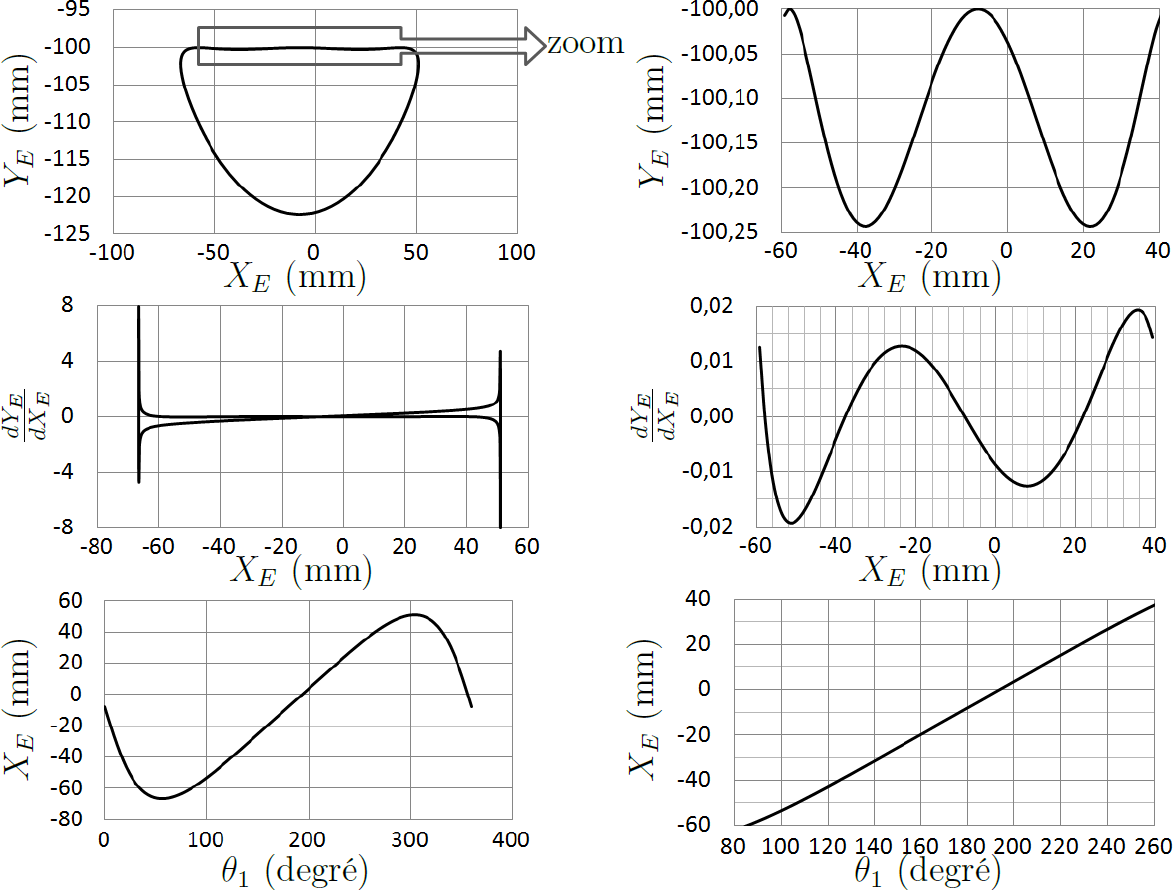
\includegraphics[width=\linewidth]{fig_03}
\textit{}
\end{center}


\subparagraph{}\textit{Compléter le graphe de structure.}% en donnant chacune des liaisons et précisant les torseurs cinématiques et statiques. }
\ifprof
\begin{corrige}~\\
\begin{center}
\begin{tabular}{|c|c|c|c|}
\hline
Liaison & Caractéristique & Torceur cinématique & Torseur statique \\
\hline\hline
$L_1 $ & Glissière de direction $\vect{x_1}$ & 
$\torseurcol{0}{0}{0}{u_1}{0}{0}{}$ & 
$\torseurcol{0}{Y_1}{Z_1}{L_1}{M_1}{N_1}{}$ \\ \hline
$L_2 $ & Rotule de centre $D$ $\vect{x_1}$ & 
$\torseurcol{p_2}{q_2}{r_2}{0}{0}{0}{D}$ & 
$\torseurcol{X_2}{Y_2}{Z_2}{0}{0}{0}{D}$ \\ \hline
$L_3 $ & Sphère--plan de normale $\left(I_1,\vect{n_1}\right)$ & 
$\torseurcol{p_3}{q_3}{r_3}{u_3}{0}{w_3}{I_1}$ & 
$\torseurcol{0}{Y_3}{0}{0}{0}{0}{I_1}$ \\ \hline
$L_4 $ & Sphère--plan de normale $\left(I_2,\vect{n_2}\right)$ & 
$\torseurcol{p_4}{q_4}{r_4}{u_4}{0}{w_4}{I_2}$ & 
$\torseurcol{0}{Y_4}{0}{0}{0}{0}{I_2}$ \\ \hline
$L_5 $ & Pivot $\left(A,\vect{z_3}\right)$ & 
$\torseurcol{0}{0}{r_5}{0}{0}{0}{A}$ & 
$\torseurcol{X_5}{Y_5}{Z_5}{L_5}{M_5}{0}{A}$ \\ \hline
$L_6 $ & Pivot $\left(B,\vect{z_3}\right)$ & 
$\torseurcol{0}{0}{r_6}{0}{0}{0}{B}$ & 
$\torseurcol{X_6}{Y_6}{Z_6}{L_6}{M_6}{0}{B}$ \\ \hline
$L_7 $ & Pivot $\left(C,\vect{z_3}\right)$ & 
$\torseurcol{0}{0}{r_7}{0}{0}{0}{C}$ & 
$\torseurcol{X_7}{Y_7}{Z_7}{L_7}{M_7}{0}{C}$ \\ \hline
\end{tabular}
\end{center}
\end{corrige}
\else
\fi

\begin{center}
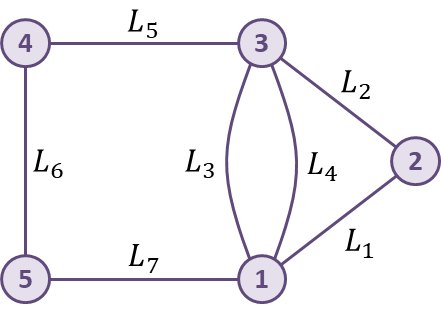
\includegraphics[width=.8\linewidth]{fig_04_bis}
%\textit{}
\end{center}

\subparagraph{}\textit{Le modèle proposé est-il isostatique ?}

\subparagraph{}\textit{Déterminer la liaison équivalente $\text{L}_{\text{eq}34}$ aux deux liaisons $\text{L}_{3}$ et $\text{L}_{4}$ situées entre le solide 1 et le solide 3. On attend une démonstration par le calcul. On précisera la forme du torseur des actions transmissibles $\mathcal{F}_{\text{eq}34}$.}
\ifprof
\begin{corrige}~\\
Les liaisons sont en parallèles, on privilégie donc la méthode statique : 
$\mathcal{F}_{\text{eq}34} =\torseurstat{T}{3}{1_{L_3}}+\torseurstat{T}{3}{1_{L_4}}$ 
$\mathcal{F}_{\text{eq}34} =\torseurl{Y_3\vect{n_1}}{\vect{0}}{O}+ \torseurl{Y_4\vect{n_2}}{\vect{0}}{O}$
$=\torseurl{Y_3\vect{n_1}+Y_4\vect{n_2}}{\vect{0}}{O}$. 

$\vect{n_1}$ et $\vect{n_2}$ ne sont pas colinéaires. $\vect{x_1}$ est orthogonal à $\vect{n_1}$  et $\vect{n_2}$. La liaison est donc une sphère cylindre d'axe $\left(O,\vect{x_1}\right)$.  
\end{corrige}
\else
\fi


\subparagraph{}\textit{Déterminer la liaison équivalente $\text{L}_{\text{eq}12}$ aux deux liaisons $\text{L}_{1}$ et $\text{L}_{2}$ situées entre le solide 1 et le solide 3. On attend une démonstration par le calcul. On précisera la forme du torseur des actions transmissibles $\mathcal{F}_{\text{eq}12}$.}
\ifprof
\begin{corrige}~\\
\end{corrige}
\else
\fi



\subparagraph{}\textit{Déterminer la liaison équivalente $\text{L}_{\text{eq}12}$ aux deux liaisons $\text{L}_{\text{eq}34}$ et $\text{L}_{\text{eq}12}$ situées entre le solide 1 et le solide 3. On attend une démonstration par le calcul. On précisera la forme du torseur des actions transmissibles $\mathcal{F}_{\text{eq}}$.
Justifier que la commande avec un seul vérin ne satisfait pas le cahier des charges.}
\ifprof
\begin{corrige}~\\
\end{corrige}
\else
\fi

\subsection*{Étude d'une commande avec deux actionneurs}
\begin{obj}
On cherche, dans un deuxième temps, à estimer la capacité d'une structure composée de deux
vérins à transmettre le mouvement attendu.
\end{obj}


\begin{center}
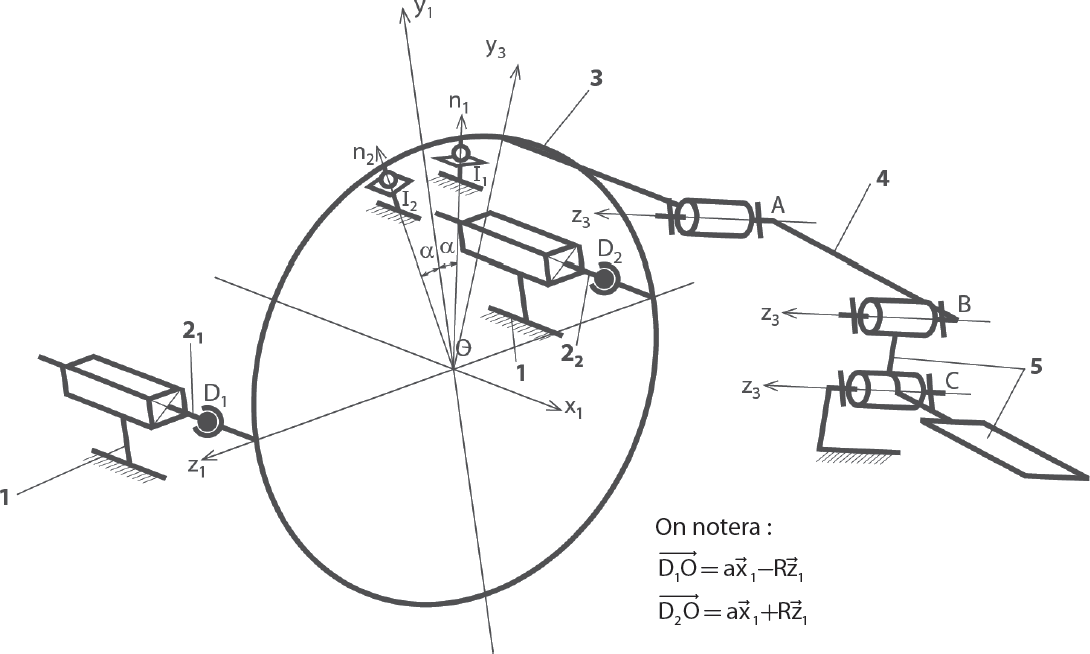
\includegraphics[width=\linewidth]{fig_05}
%\textit{}
\end{center}

\subparagraph{}\textit{À partir du graphe de structure (graphe des liaisons) et en vous inspirant des résultats trouvés précédemment déterminer la liaison équivalente $\text{L}_{\text{eq}1}$
aux liaisons $\text{L}_{11}$, $\text{L}_{21}$ et la liaison équivalente $\text{L}_{\text{eq}2}$ aux liaisons $\text{L}_{12}$ et $\text{L}_{22}$ entre les solides 1 et 3.}
\ifprof
\begin{corrige}~\\
\end{corrige}
\else
\fi


\subparagraph{}\textit{Déterminer par la méthode de votre choix, la liaison équivalente $\text{L'}_{\text{eq}1}$ aux deux liaisons $\text{L}_{\text{eq}34}$, $\text{L}_{\text{eq}1}$ et $\text{L}_{\text{eq}2}$ situées
entre le solide 1 et le solide 3. On précisera la forme du torseur des actions transmissibles $\mathcal{F}'_{\text{eq}}$ puis le torseur cinématique cinématique $\mathcal{V}'_{\text{eq}}$. Le cahier des charges est-il vérifié pour une commande avec deux vérins ?}
\ifprof
\begin{corrige}~\\
\end{corrige}
\else
\fi

\subsection*{Étude de la structure adoptée par le constructeur}
\begin{obj}
On cherche finalement à estimer la capacité de réalisation d'une structure composée des quatre
vérins.
\end{obj}





\subparagraph{}\textit{Pour des raisons d'encombrement des vérins et de capacité à fournir les actions mécaniques de poussée, le
bureau d'étude a finalement choisi de commander le tore avec 4 vérins pour obtenir la liaison glissière
comme liaison équivalente entre les solides 1 et 3. Quel est, dans ces conditions, le degré d'hyperstatisme du
groupe de liaisons initial réalisant la liaison glissière ? Vous expliquerez brièvement, mais clairement votre
raisonnement. Que pensez vous de ce résultat sur la capacité de réalisation de cette structure ?}
\ifprof
\begin{corrige}~\\
\end{corrige}
\else
\fi

\ifprof
\else
\end{multicols}
\fi
%\includepdf[pages=-]{OLD_Corrige.pdf}
